% mainfile: ../../../../master.tex
\subsection{DNA and RNA quantification with NanoDrop\cR ND-1000 Spectrophotometer}
% The part of the label after the colon must match the file name. Otherwise,
% conditional compilation based on task labels does NOT work.
\label{task:20180313_cj0}
\tags{lab,qnt,dna,rna}
\authors{cj}
\files{ndv\_to\_latex\_tab.py}
%\persons{}

% Figures
\begin{figure}[H] % position of the figure 
    \centering
    \caption{NanoDrop spectra for DNA and RNA isolated with MasterPure\texttrademark~ Kit}
    \label{fig:label}
    \begin{subfigure}[b]{0.3\textwidth}
        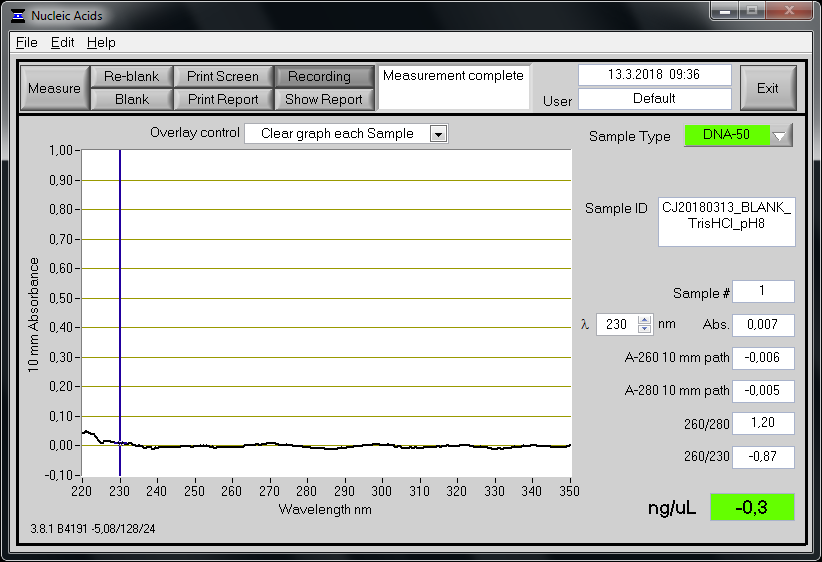
\includegraphics[width=\textwidth]{graphics/screenshots/CJ20180313_BLANK_TrisHCl_pH8.png}
        \caption{Spectrum of the Tris-HCl buffer pH 8 used as Blank}
        \label{sfig:CJ20180313_BLANK_TrisHCl_pH8}
    \end{subfigure}
    ~ 
    \begin{subfigure}[b]{0.3\textwidth}
        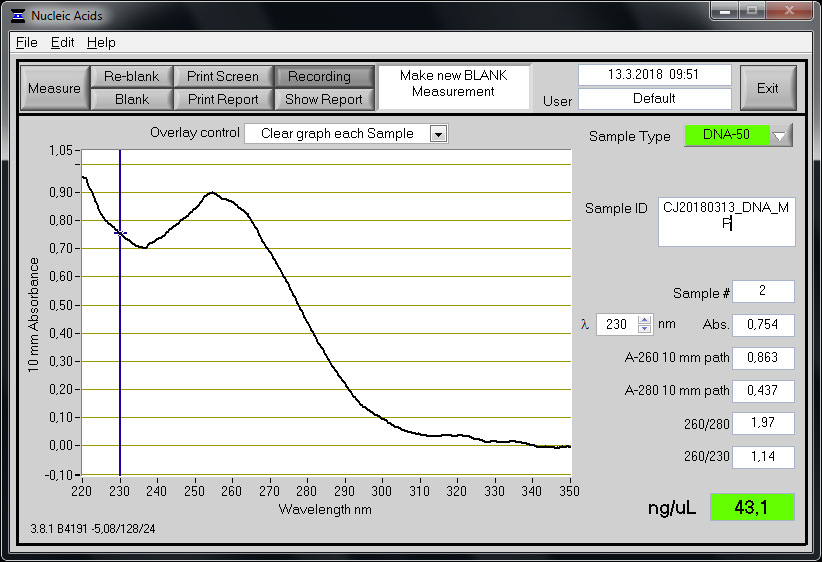
\includegraphics[width=\textwidth]{graphics/screenshots/CJ20180313_DNA_MP.png}
        \caption{Spectrum of the DNA extracted with MasterPure\texttrademark~ kit}
        \label{sfig:CJ20180313_DNA_MP}
    \end{subfigure}
    ~ 
    \begin{subfigure}[b]{0.3\textwidth}
        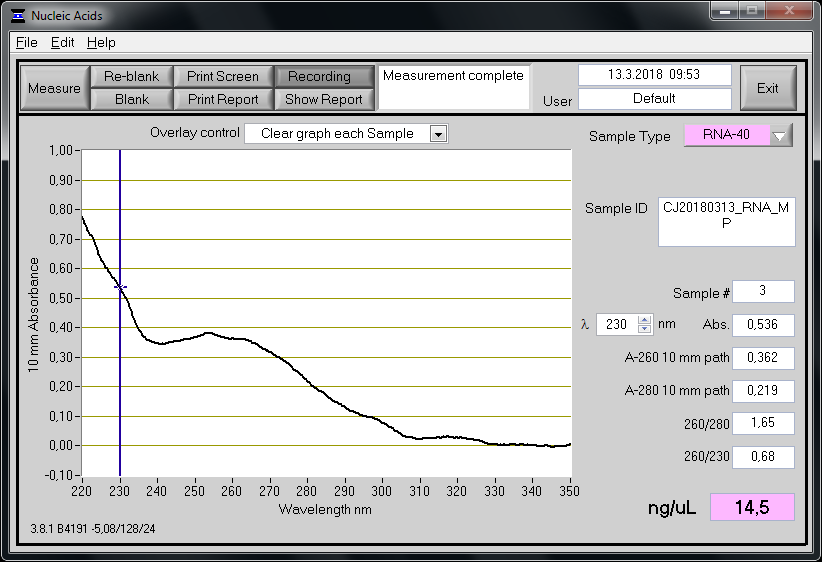
\includegraphics[width=\textwidth]{graphics/screenshots/CJ20180313_RNA_MP.png}
        \caption{Spectrum of the RNA extracted with MasterPure\texttrademark~ kit}
        \label{sfig:CJ20180313_RNA_MP}
    \end{subfigure}
\end{figure}

\begin{table}[htbp]
\caption{CJ20180313.txt}
\label{tab:}
\centering
\begin{tabular}{l l l l l l l l l l l l l }
\toprule
Sample ID & Time  & ng/ul  & A260  & A280  & 260/280  & 260/230  \\ \midrule
\texttt{CJ20180313\_BLANK\_TrisHCl\_pH8} & 09:35 & -0,32 & -0,006 & -0,005 & 1,20 & -0,87 \\
\texttt{CJ20180313\_DNA\_MP} & 09:37 & 43,13 & 0,863 & 0,437 & 1,97 & 1,14 \\
\texttt{CJ20180313\_RNA\_MP} & 09:53 & 14,49 & 0,362 & 0,219 & 1,65 & 0,68 \\
\bottomrule
\end{tabular}
\\
User: Default - Date: 13.3.2018 - Constant: 40,00 - Cursor position: 230 \
\end{table}
